\documentclass[border=2pt]{standalone}
\usepackage{tikz}
\usetikzlibrary{arrows.meta}

\begin{document}
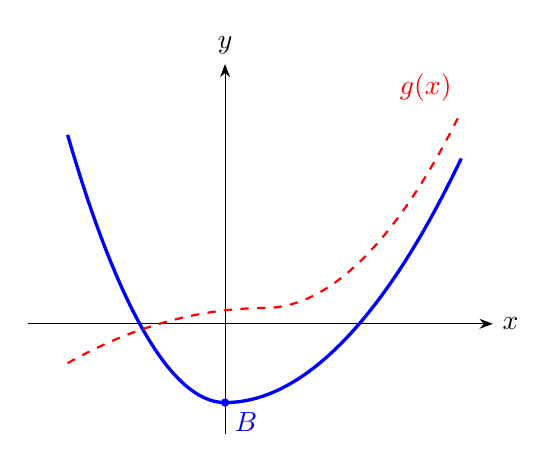
\begin{tikzpicture}[x=1cm, y=1cm, >=Stealth]
  \draw[->] (-2.5,0) -- (3.4,0) node[right] {$x$};
  \draw[->] (0,-1.4) -- (0,3.3) node[above] {$y$};

  \draw[blue, very thick]
    (-2,2.4) parabola bend (0,-1) (3,2.1);
  \fill[blue] (0,-1) circle (1.5pt);
  \node[below right, blue] at (0,-1) {$B$};

  \draw[red, thick, dashed]
    (-2,-.5) parabola[bend={(.5,.2)}] (3,2.7);
  \node[red, above left] at (3,2.7) {$g(x)$};
\end{tikzpicture}
\end{document}
